\documentclass[twoside]{article}
\setlength{\oddsidemargin}{0.25 in}
\setlength{\evensidemargin}{-0.25 in}
\setlength{\topmargin}{-0.6 in}
\setlength{\textwidth}{6.5 in}
\setlength{\textheight}{8.5 in}
\setlength{\headsep}{0.75 in}
\setlength{\parindent}{0 in}
\setlength{\parskip}{0.1 in}

\usepackage{graphicx}
\usepackage{url}

%
% The following commands sets up the lecnum (lecture number)
% counter and make various numbering schemes work relative
% to the lecture number.
%
\newcounter{lecnum}
\renewcommand{\thepage}{\thelecnum-\arabic{page}}
\renewcommand{\thesection}{\thelecnum.\arabic{section}}
\renewcommand{\theequation}{\thelecnum.\arabic{equation}}
\renewcommand{\thefigure}{\thelecnum.\arabic{figure}}
\renewcommand{\thetable}{\thelecnum.\arabic{table}}
\newcommand{\dnl}{\mbox{}\par}

%
% The following macro is used to generate the header.
%
\newcommand{\lecture}[4]{
  \pagestyle{myheadings}
  \thispagestyle{plain}
  \newpage
  \setcounter{lecnum}{#1}
  \setcounter{page}{1}
  \noindent
  \begin{center}
  \framebox{
     \vbox{\vspace{2mm}
   \hbox to 6.28in { {\bf CMPSCI~630~~~ Systems
                       \hfill Spring 2018} }
      \vspace{4mm}
      \hbox to 6.28in { {\Large \hfill Lecture #1  \hfill} }
%       \hbox to 6.28in { {\Large \hfill Lecture #1: #2  \hfill} }
      \vspace{2mm}
      \hbox to 6.28in { {\it Lecturer: #3 \hfill Scribe: #4} }
     \vspace{2mm}}
  }
  \end{center}
  \markboth{Lecture #1: #2}{Lecture #1: #2}
  \vspace*{4mm}
}

%
% Convention for citations is authors' initials followed by the year.
% For example, to cite a paper by Leighton and Maggs you would type
% \cite{LM89}, and to cite a paper by Strassen you would type \cite{S69}.
% (To avoid bibliography problems, for now we redefine the \cite command.)
%
\renewcommand{\cite}[1]{[#1]}

% \input{epsf}

%Use this command for a figure; it puts a figure in wherever you want it.
%usage: \fig{NUMBER}{FIGURE-SIZE}{CAPTION}{FILENAME}
\newcommand{\fig}[4]{
           \vspace{0.2 in}
           \setlength{\epsfxsize}{#2}
           \centerline{\epsfbox{#4}}
           \begin{center}
           Figure \thelecnum.#1:~#3
           \end{center}
   }

% Use these for theorems, lemmas, proofs, etc.
\newtheorem{theorem}{Theorem}[lecnum]
\newtheorem{lemma}[theorem]{Lemma}
\newtheorem{proposition}[theorem]{Proposition}
\newtheorem{claim}[theorem]{Claim}
\newtheorem{corollary}[theorem]{Corollary}
\newtheorem{definition}[theorem]{Definition}
\newenvironment{proof}{{\bf Proof:}}{\hfill\rule{2mm}{2mm}}

% Some useful equation alignment commands, borrowed from TeX
\makeatletter
\def\eqalign#1{\,\vcenter{\openup\jot\m@th
 \ialign{\strut\hfil$\displaystyle{##}$&$\displaystyle{{}##}$\hfil
     \crcr#1\crcr}}\,}
\def\eqalignno#1{\displ@y \tabskip\@centering
 \halign to\displaywidth{\hfil$\displaystyle{##}$\tabskip\z@skip
   &$\displaystyle{{}##}$\hfil\tabskip\@centering
   &\llap{$##$}\tabskip\z@skip\crcr
   #1\crcr}}
\def\leqalignno#1{\displ@y \tabskip\@centering
 \halign to\displaywidth{\hfil$\displaystyle{##}$\tabskip\z@skip
   &$\displaystyle{{}##}$\hfil\tabskip\@centering
   &\kern-\displaywidth\rlap{$##$}\tabskip\displaywidth\crcr
   #1\crcr}}
\makeatother

% **** IF YOU WANT TO DEFINE ADDITIONAL MACROS FOR YOURSELF, PUT THEM HERE:



% Some general latex examples and examples making use of the
% macros follow.

\begin{document}

%FILL IN THE RIGHT INFO.
%\lecture{**LECTURE-NUMBER**}{**DATE**}{**LECTURER**}{**SCRIBE**}
\lecture{6}{February 14}{Emery Berger}{Angela Upreti}

\section{Interlude: Software Architecture}
In a client-server architecture and other time sharing architectures, virtual memory(VMM) allows the illusion that every client has all of the address space. In most systems, memory is virtually tagged and caches are physically tagged. Cloud service providers such as amazon take advantage of VMM and VMs to provide a seemingly isolated environment to their clients. They also guarantee timely execution which means an appropriate scheduling is necessary to meet this guarantee.  We talked about naive round-robin scheduling and why round-robin would not be enough.  
\section{Context Switch}
Time-slicing allows efficient use of the processors. If a process running on a processor is I/O bound, the idle cpu time can be used by another process. Before switching to another process, the current processor state has to be saved and another process's state has to be restored.This has a lot of overhead because context switch involves crossing the kernel boundary. 

\textbf{Overheads of a Context Switch }
\begin{enumerate}
\item Registers
\item Vector Registers
\item Program Counter
\item TLB : Page table maps virtual memory space to physical address. TLB is like a cache of the page table. It stores recently accessed virtual memory addresses. It is much faster than looking up the page table. x-86 page table is stored as a radix tree which is expensive to trace in case of a cache miss. Every core has its own TLB. Whenever, a page table is modified by one of the processes, the TLB entries storing that mapping need to be invalidated for all processors. This is expensive. 
While discussing the TLB, we talked about the possibility of a shared TLB and other shared resources. Isolating resources between processors would provide better security but resources might go under utilized. 
\item Cross-kernel boundary 
\end{enumerate}
\textbf{Timeline of a context switch }
\begin{enumerate}
 \item A process ${P_1}$ does a system call.
 \item ${P_1}$ is waiting in the queue for execution.
 \item  $P_1$ joins the ready queue after it is signaled. 
\end{enumerate}
 
 If we have two processes $P_1$ and $P_2$, \\
 
\begin{center}
                $P_1$---------------- $t(q_1)$ --------------------$P_2$-----------------------\\
               \end{center}               
If $q_1$ is too long , memory is cold for $P_2$.  \\
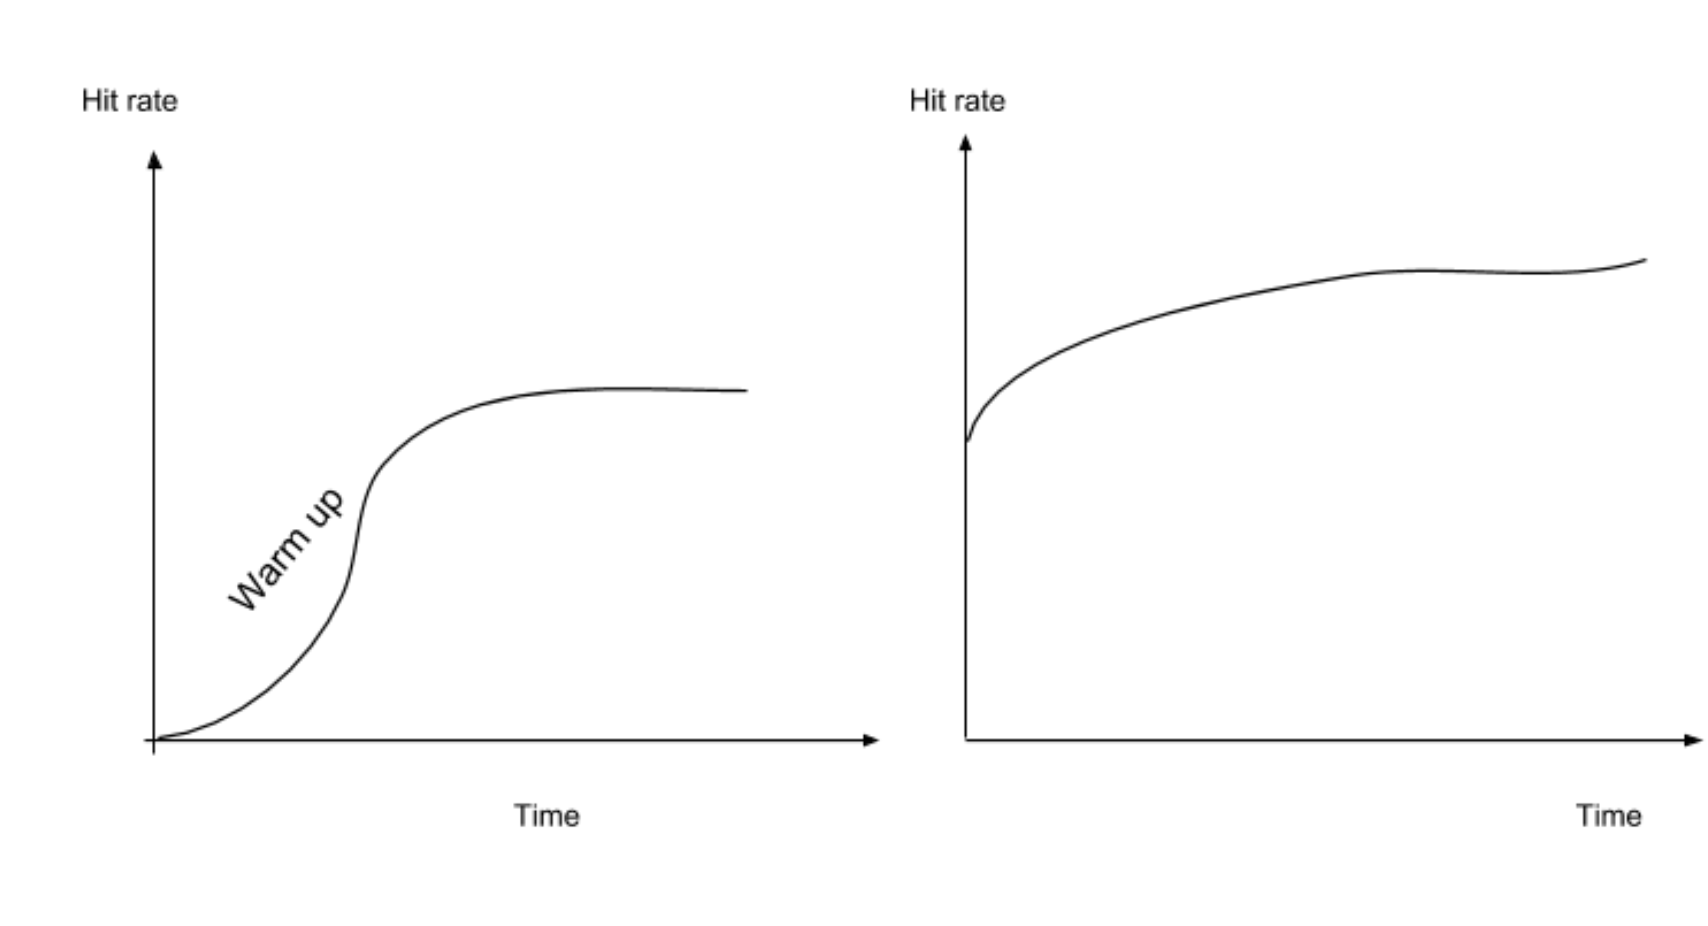
\includegraphics[width=\textwidth]{cachehitrate}
 
The image on the left shows the phase where the cache warms up at the beginning and achieves an optimal hit rate. The image on the left eliminates the warm-up rate. This can be achieved by sharing memory pages between processes.  
 
 \textbf{Time Quantum length }
 
Related to duration that a page stays in cache is the value of time quantum. A long time quantum provides higher throughput and a smaller quantum provides lower latency. Long time quantum will likely make better use of pages cache. 
\section{Scheduling}
\subsection{Priority-based Schedulers }: This is a multi-level preemptive scheduling policy. There are multiple ready queues and each queue has a priority level assigned to it. The queue with the highest priority is scheduled first. A round-robin scheduling is used within a queue. 
Priority-based scheduling can lead to starvation. If a process with a higher priority is always present, a low-priority process might never run. Real-time applications cannot use priority based scheduling. 
\subsection{Proportional Share Schedulers}
These are based on lottery tickets. All processes get some lottery tickets. The number of tickets a process gets is based on the proportion of  cpu time we want to allot it. A lottery ticket would be randomly sampled. This randomness in scheduling provides better security. \\
\textbf{Independence}: Between two sampled elements $s_i$ and  $s_j$  $\in  S$, $corr(s_i ,s_j) = 0 $.
\textbf{Cryptographically secure }: Given samples $s_0,  s_1, s_2,...,s_n$, one cannot figure out $s_{n+1}$. 
\subsection{Scheduling-bases on Deadlines} 
Earliest deadline first would be an example of this. 
\subsection{Boosting}  
Processes with higher CPU utilization get higher priority. I/O bound processes get a lower priority. This leads to really good CPU utilization.
\subsection{QoS Guarantee} An example would be `10 percent of the time every window of 100ms with a probability of 0.9.'
\end{document}
